%!TEX root = ../thesis.tex
\chapter{News-Media organisation Twitter activity \label{app:activity}}

This appendix includes the tweet activity over the 2019 calendar year for a select group of representative news-media organisations. In each figure, a red line at 5 tweets per day is shown as a reference for comparison between accounts. The full collection of 154 news-media organisations can be accessed online via figshare~\cite{figshareSouth2021}.
\captionsetup[figure]{list=no,hypcap=false}

% \newpage

% \subsubsection{The three largest news-media organisations by follower count}

% These large organisations produce a wealth of content that is viewed by a large number of consumers. While these organisations slow down entropy estimation, they easily converge.

% \begin{center}

% 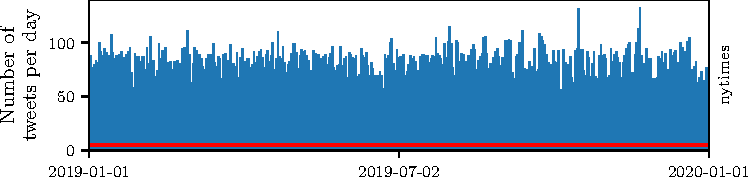
\includegraphics{appendix2/figs/tweet_times/nytimes.pdf}
% \captionof{figure}{Twitter activity over 2019 for `The New York Times' with 44800317 followers and 31029 total tweets. 
%  Red line is 5 tweets per day.}
% \end{center}



% \begin{center}

% 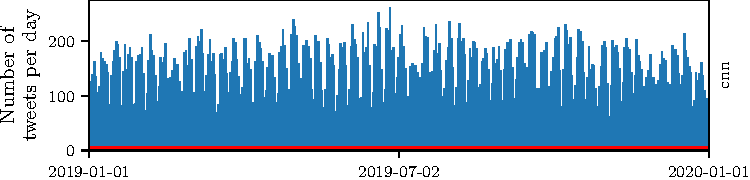
\includegraphics{appendix2/figs/tweet_times/cnn.pdf}
% \captionof{figure}{Twitter activity over 2019 for `CNN' with 44153462 followers and 57155 total tweets. 
%  Red line is 5 tweets per day.}
% \end{center}



% \begin{center}

% 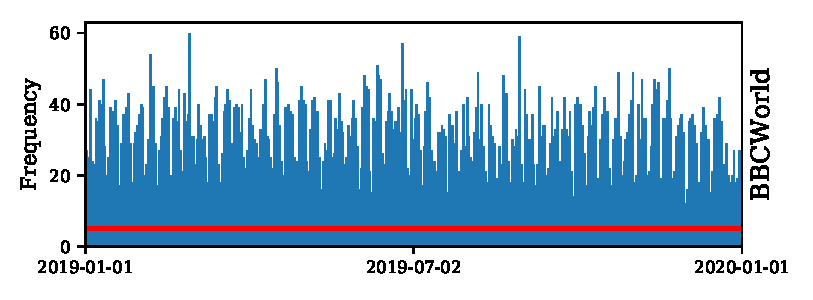
\includegraphics{appendix2/figs/tweet_times/BBCWorld.pdf}
% \captionof{figure}{Twitter activity over 2019 for `BBC News (World)' with 26446876 followers and 11679 total tweets. 
%  Red line is 5 tweets per day.}
% \end{center}

% \newpage
% \subsubsection{The three smallest news-media organisations by follower count}
% Although follower count 

% \begin{center}

% 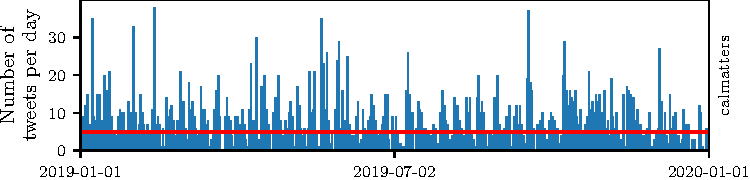
\includegraphics{appendix2/figs/tweet_times/calmatters.pdf}
% \captionof{figure}{Twitter activity over 2019 for `CalMatters' with 15069 followers and 3247 total tweets. 
%  Red line is 5 tweets per day.}
% \end{center}



% \begin{center}

% 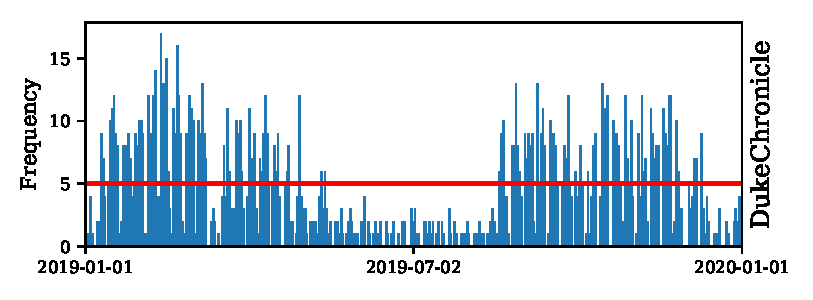
\includegraphics{appendix2/figs/tweet_times/DukeChronicle.pdf}
% \captionof{figure}{Twitter activity over 2019 for `The Chronicle' with 15207 followers and 1537 total tweets. 
%  Red line is 5 tweets per day.}
% \end{center}




% \begin{center}

% 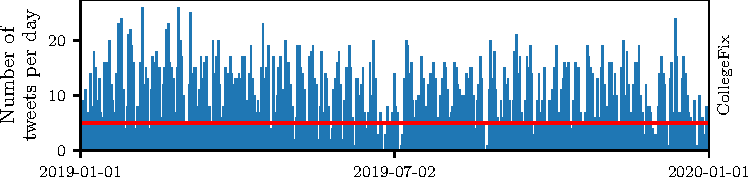
\includegraphics{appendix2/figs/tweet_times/CollegeFix.pdf}
% \captionof{figure}{Twitter activity over 2019 for `The College Fix' with 15289 followers and 4094 total tweets. 
%  Red line is 5 tweets per day.}
% \end{center}


\subsubsection{The news-media organisations with the largest number of tweets}

These large organisations produce a wealth of content that is viewed by a large number of consumers. While these organisations slow down entropy estimation, they easily converge.


\begin{center}

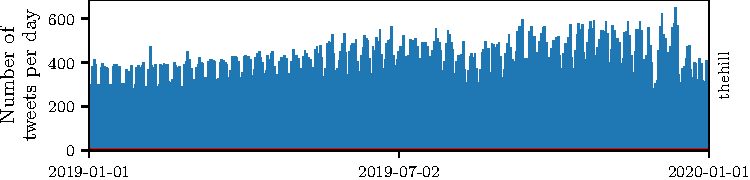
\includegraphics{appendix2/figs/tweet_times/thehill.pdf}
\captionof{figure}{Twitter activity over 2019 for `The Hill' with 3501890 followers and 157172 total tweets. 
 Red line is 5 tweets per day.}
\end{center}

\begin{center}

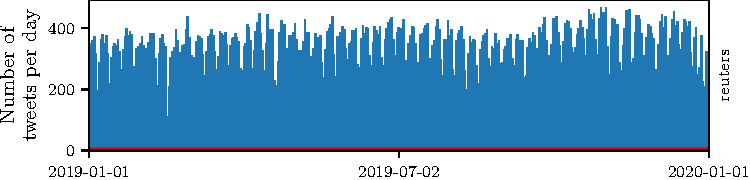
\includegraphics{appendix2/figs/tweet_times/reuters.pdf}
\captionof{figure}{Twitter activity over 2019 for `Reuters' with 21042215 followers and 128448 total tweets. 
 Red line is 5 tweets per day.}
\end{center}


\begin{center}

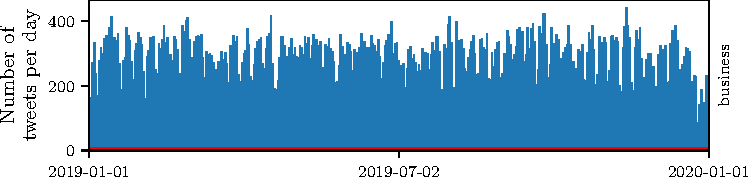
\includegraphics{appendix2/figs/tweet_times/business.pdf}~
\captionof{figure}{Twitter activity over 2019 for `Bloomberg' with 5790419 followers and 109367 total tweets. 
 Red line is 5 tweets per day.}
\end{center}



\subsubsection{The news-media organisations with the smallest number of tweets}

These news organisations are the smallest tweet counts that have passed through our filtering processes. Each organisation here exemplifies abnormalities that are exhibited by many of these low activity organisations. \autoref{app:fig:TheLibRepublic} shows both the low overall activity (which makes entropy rate estimation difficult) and the presence of large spikes in activity, \autoref{app:fig:sciencedaily} shows a sustained low activity over the year, with clear weekend dips in activity, and \autoref{app:fig:Commentary} show a initial period of low activity paired with a later period of higher activity starting in August.

% \captionsetup[figure]{list=no,hypcap=true}
\begin{center}

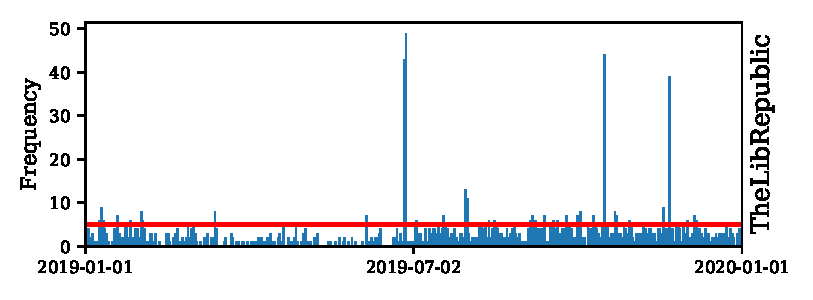
\includegraphics{appendix2/figs/tweet_times/TheLibRepublic.pdf}
\captionof{figure}{Twitter activity over 2019 for `Libertarian Republic' with 47475 followers and 1145 total tweets. 
 Red line is 5 tweets per day.}\label{app:fig:TheLibRepublic}
\end{center}

\begin{center}

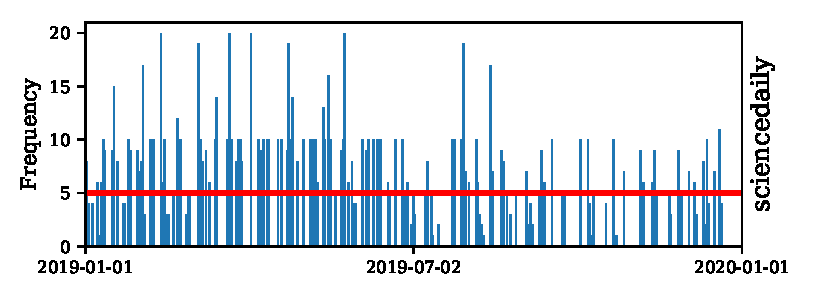
\includegraphics{appendix2/figs/tweet_times/sciencedaily.pdf}
\captionof{figure}{Twitter activity over 2019 for `ScienceDaily' with 240013 followers and 1243 total tweets. 
 Red line is 5 tweets per day.}\label{app:fig:sciencedaily}
\end{center}{}

\begin{center}

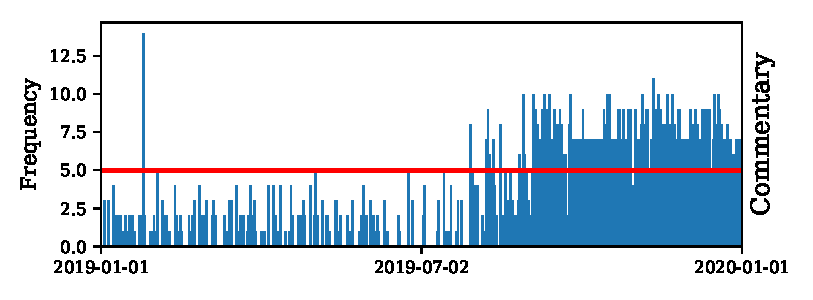
\includegraphics{appendix2/figs/tweet_times/Commentary.pdf}
\captionof{figure}{Twitter activity over 2019 for `Commentary Magazine' with 35704 followers and 1337 total tweets. 
 Red line is 5 tweets per day.}\label{app:fig:Commentary}
\end{center}














